\documentclass[11pt,a4paper]{article}
\usepackage[utf8]{inputenc}
\usepackage[T1]{fontenc}
\usepackage{geometry}
\geometry{margin=2.4cm}
\usepackage{xcolor}
\usepackage{tikz}
\usetikzlibrary{arrows.meta, positioning, fit, calc, backgrounds}
\usepackage{booktabs}
\usepackage{tabularx}
\usepackage{enumitem}
\usepackage{hyperref}
\usepackage{fancyhdr}
\usepackage{titlesec}
\usepackage{tcolorbox}
\tcbuselibrary{skins, breakable}
\usepackage{float}

% Colours
\definecolor{sub}{RGB}{30, 60, 114}
\definecolor{acc}{RGB}{190, 60, 50}
\definecolor{grn}{RGB}{46, 139, 87}
\definecolor{vio}{RGB}{120, 80, 160}

% Header
\pagestyle{fancy}
\fancyhf{}
\fancyhead[L]{\small\textcolor{sub}{\textbf{Substrate House}}}
\fancyhead[R]{\small\textcolor{sub}{Proposal B}}
\fancyfoot[C]{\thepage}
\renewcommand{\headrulewidth}{0.4pt}
\renewcommand{\headrule}{\hbox to\headwidth{\color{sub}\leaders\hrule height \headrulewidth\hfill}}

\titleformat{\section}{\large\bfseries\color{sub}}{\thesection}{1em}{}[\vspace{-0.5em}\textcolor{sub}{\rule{\textwidth}{0.3pt}}]
\titleformat{\subsection}{\normalsize\bfseries\color{sub!80}}{\thesubsection}{1em}{}

\setlength{\parskip}{0.45em}
\setlength{\parindent}{0pt}

\title{%
  \textcolor{sub}{\rule{\textwidth}{1.2pt}}\\[0.4cm]
  {\LARGE\bfseries\textcolor{sub}{Soba}}\\[0.1cm]
  {\large\textcolor{sub!60}{The fast path: an existing robot, fine-tuned models, 8 weeks}}\\[0.3cm]
  \textcolor{sub}{\rule{\textwidth}{1.2pt}}
}
\author{\textbf{Substrate House} \textperiodcentered\ London}
\date{April 2026}

\begin{document}
\maketitle
\thispagestyle{fancy}

% ──────────────────────────────────────────────────────────────────────────────
\section{The argument for going fast}

Proposal A describes building Soba as a humanoid. It's the more ambitious version: full-body expression, our own foundation model, a Unitree G1 walking around the room. It's also 16 weeks, \pounds 18k, and carries real engineering risk around the G1's SDK maturity and walking-near-humans safety.

This proposal asks a different question: \emph{what is the fastest credible version of Soba we can put in front of a person?}

The answer is to take a robot that already exists and already knows how to express affect --- and wire it up to our biosignal pipeline. We skip mechanical integration entirely. We use fine-tuned open-source models instead of waiting for our foundation model to be production-ready. We get a working closed-loop demo in 8 weeks for under \pounds 5k. And critically, we get to answer the question that matters most before investing further: \emph{does biosignal-driven robot adaptation actually change how people feel?}

If the answer is yes, we build Proposal A with confidence. If the answer is more complicated --- if people find it creepy, or if the latency is too high for the effect to register, or if the model's state estimates aren't reliable enough --- we learn that at \pounds 5k instead of \pounds 20k.

% ──────────────────────────────────────────────────────────────────────────────
\section{Choosing the robot}

We considered every social robot platform currently available for purchase. Most of them are dead or dying. Jibo and Kuri are gone. Pepper's production was halted in 2021. Aldebaran (NAO, Pepper) entered receivership in mid-2025 and was acquired by Maxtronics --- we don't want to bet on a platform with uncertain long-term support. Misty Robotics shut down in 2023.

That leaves two serious options, and they represent genuinely different design philosophies.

\subsection{Furhat: the face}

Furhat is a stationary bust that projects an animated face onto a 3D-printed mask. The face is photorealistic: it does lip sync, gaze tracking, eyebrow raises, micro-expressions. It is, by a wide margin, the most expressive face in commercial social robotics. It has a 3-DOF neck, a speaker, a mic array, and a well-documented REST API that we can call from Python.

The price is quote-based, roughly \pounds 20--25k for a research license. It doesn't move. It sits on a table and looks at you.

For our stationary recording configuration --- where the participant is seated, wearing EEG and eye tracking, with fNIRS and StretchSense --- Furhat is a natural fit. The participant is already still. The robot doesn't need to approach or retreat; it communicates entirely through its face and voice. And the face is the single strongest channel for communicating empathy: a slow blink, a slight head tilt, a softened expression. Humans are exquisitely sensitive to faces. Furhat exploits this.

\begin{table}[H]
\centering\small
\begin{tabularx}{\textwidth}{lX}
\toprule
Expression & Back-projected animated face, lip sync, gaze direction, micro-expressions \\
Movement & 3-DOF neck (pan, tilt, roll) \\
Audio & Speaker, 3-mic array, built-in ASR and TTS \\
SDK & Kotlin SDK, REST API, visual dialogue builder \\
Price & $\sim$\pounds 20k--25k (research, quote-based) \\
Link & \url{https://furhatrobotics.com/get-furhat} \\
\bottomrule
\end{tabularx}
\end{table}

\subsection{MiRo-E: the animal}

MiRo-E is a small biomimetic robot built by \href{https://www.miro-e.com}{Consequential Robotics} in Sheffield. It looks like a simplified rabbit or dog --- ears that move, LED eyes, a tail, a wheeled base. It costs \pounds 2,450. It has touch sensors on its head and body, stereo cameras, four microphones, and sonar. It was designed from the ground up for affective interaction research.

MiRo-E's advantage over Furhat is mobility. It can approach and retreat, which is one of the most powerful behavioural signals we want to use: proximity modulation driven by the person's arousal and stress. Its animal form also sidesteps the uncanny valley entirely. Nobody expects a robot rabbit to have a human face. When it flattens its ears and backs away because you're stressed, that reads as ``the creature is responding to you'' rather than ``the mannequin is performing empathy.''

Its limitation is expressive resolution. LED eyes and ear angles carry less information than Furhat's projected face. We partially compensate with sound (tones, chirps, breathing rhythms) from an external speaker.

\begin{table}[H]
\centering\small
\begin{tabularx}{\textwidth}{lX}
\toprule
Expression & LED eyes, ear movement (2 DOF each), tail, body posture, head pitch/yaw/lift \\
Movement & Wheeled base, omnidirectional \\
Sensors & Stereo cameras, 4 mics, touch sensors (head + body), sonar, cliff sensors \\
SDK & Python SDK, ROS1 (ROS2 via community bridge) \\
Price & \pounds 2,450 \\
Link & \url{https://www.miro-e.com} \\
\bottomrule
\end{tabularx}
\end{table}

\subsection{Our recommendation}

Start with MiRo-E. It gives us mobility, it's cheap, it's UK-based (easy procurement, no import delays), and we can have it running in days. Use it to build the full pipeline and run the first user studies. If the results warrant a richer expressive channel, add Furhat for the stationary configuration. The two robots serve different recording setups anyway: MiRo-E for mobile, Furhat for stationary.

% ──────────────────────────────────────────────────────────────────────────────
\section{The model: fine-tuning, not training from scratch}

Our foundation model is the long-term goal. But it doesn't need to be ready for this version of Soba. Open-source models for EEG decoding, HRV analysis, and speech emotion recognition have matured to the point where fine-tuning them on our data will get us a usable state vector in weeks rather than months.

The architecture is simple: separate feature extractors per modality, feeding into a small fusion layer that outputs the state vector.

\begin{figure}[H]
\centering
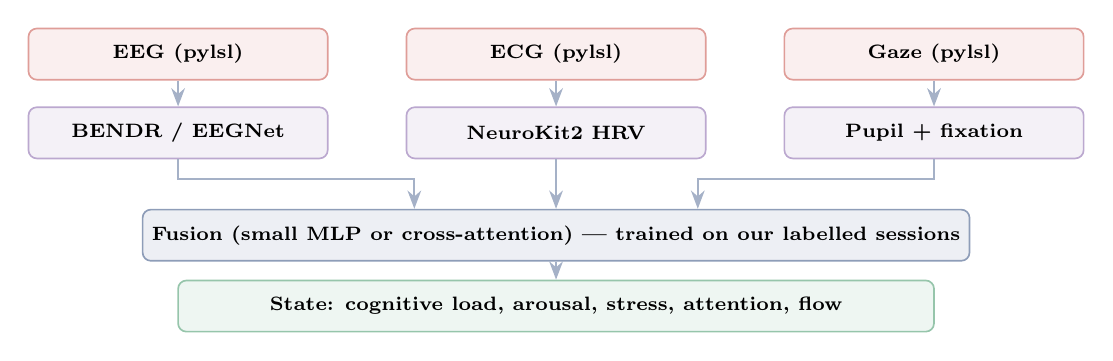
\begin{tikzpicture}[
    >=Stealth, node distance=0.5cm,
    mod/.style={rectangle, rounded corners=3pt, draw=#1!50, fill=#1!8,
      minimum width=3.8cm, minimum height=0.65cm, align=center,
      font=\scriptsize\bfseries, line width=0.6pt},
    arr/.style={->, thick, sub!40}
  ]
  \node[mod=acc] (eeg) at (0, 2.8) {EEG (pylsl)};
  \node[mod=vio] (eegm) at (0, 1.8) {BENDR / EEGNet};

  \node[mod=acc] (ecg) at (4.8, 2.8) {ECG (pylsl)};
  \node[mod=vio] (ecgm) at (4.8, 1.8) {NeuroKit2 HRV};

  \node[mod=acc] (eye) at (9.6, 2.8) {Gaze (pylsl)};
  \node[mod=vio] (eyem) at (9.6, 1.8) {Pupil + fixation};

  \node[mod=sub, minimum width=9.6cm] (fusion) at (4.8, 0.5)
    {Fusion (small MLP or cross-attention) --- trained on our labelled sessions};

  \node[mod=grn, minimum width=9.6cm] (out) at (4.8, -0.4)
    {State: cognitive load, arousal, stress, attention, flow};

  \draw[arr] (eeg) -- (eegm);
  \draw[arr] (ecg) -- (ecgm);
  \draw[arr] (eye) -- (eyem);
  \draw[arr] (eegm.south) -- ++(0,-0.25) -| ([xshift=-1.8cm]fusion.north);
  \draw[arr] (ecgm.south) -- ++(0,-0.25) -- (fusion.north);
  \draw[arr] (eyem.south) -- ++(0,-0.25) -| ([xshift=1.8cm]fusion.north);
  \draw[arr] (fusion) -- (out);
\end{tikzpicture}
\caption{Per-modality feature extractors feed a lightweight fusion layer. The whole thing trains in hours on a single GPU.}
\end{figure}

The key models:

\textbf{BENDR} (\href{https://github.com/SPOClab-ca/BENDR}{github.com/SPOClab-ca/BENDR}) is a pre-trained EEG transformer --- essentially BERT for brainwaves, trained on the Temple University Hospital EEG corpus. We fine-tune it on our labelled recording sessions to predict cognitive load and arousal from EEG windows. If BENDR proves too heavy for real-time inference, we fall back to \textbf{EEGNet} (\href{https://github.com/vlawhern/arl-eegmodels}{github.com/vlawhern/arl-eegmodels}), a compact CNN that runs comfortably on edge hardware.

\textbf{NeuroKit2} (\href{https://github.com/neuropsychology/NeuroKit}{github.com/neuropsychology/NeuroKit}) handles ECG and EDA feature extraction --- not a neural network, just well-tested signal processing. It gives us RMSSD, LF/HF ratio, pNN50, SCR peaks, and tonic conductance level. These are the standard features; the fusion layer learns what to weight.

\textbf{Py-FEAT} (\href{https://github.com/cosanlab/py-feat}{github.com/cosanlab/py-feat}) runs on the robot's camera to detect the participant's facial action units and emotional expression. This is a second channel of affect information that doesn't require the person to wear anything.

The fusion layer is a small MLP (or, if we have enough labelled data, a cross-attention module). A few hundred thousand parameters. It takes the concatenated feature vectors from all modalities and outputs the five-dimensional state vector. We train it on our labelled recording sessions with a simple regression loss against annotated cognitive/affective states. The pipeline is designed so that when our foundation model is ready, we swap it in as a drop-in replacement --- the fusion layer and per-modality extractors get replaced by a single model, but the rest of the system (LSL receiver, preprocessing, behaviour policy, robot control) stays identical.

% ──────────────────────────────────────────────────────────────────────────────
\section{How Soba behaves}

The same five state dimensions as Proposal A, but the output channels are different.

\begin{table}[H]
\centering\small
\begin{tabularx}{\textwidth}{lXX}
\toprule
\textbf{When this is high} & \textbf{Furhat} & \textbf{MiRo-E} \\
\midrule
Cognitive load & Slow speech rate. Simplify expression to neutral. Pause between utterances. Reduce head movement. & Slow to a stop. Dim LEDs. Flatten ears. Become small and quiet. \\
Arousal & Calm expression. Slow blinks. Softer voice. Slight head tilt (listening posture). & Still body. Tail down. Slow, rhythmic ear movement. Breathing-rate LED pulse. \\
Low attention & Direct gaze at person. Raise eyebrows. Verbal prompt (``still with me?''). & Drive forward slightly. Perk ears. Short chirp sound. \\
Stress & Empathetic expression. Slow nod. Lower pitch. & Back away. Lower head. Slow blue LED pulse (4\,s cycle). \\
Flow & \textbf{Neutral face. Silence. Wait.} & \textbf{Freeze. Dim everything. Do not move until flow breaks.} \\
\bottomrule
\end{tabularx}
\end{table}

The MiRo-E behaviours are deliberately animal-like. When the person is stressed, MiRo-E doesn't try to look empathetic --- it shrinks, retreats, goes quiet. The behavioural metaphor is a sensitive animal that can read the room. This works because it's congruent with the form factor: people don't expect a robot rabbit to say ``I understand you're stressed,'' but they do read its withdrawal as a social signal.

The same design principles apply as in Proposal A: smooth interpolation between states, hysteresis to prevent oscillation, and a hard gate for flow preservation.

% ──────────────────────────────────────────────────────────────────────────────
\section{Timeline}

\begin{table}[H]
\centering\small
\begin{tabularx}{\textwidth}{clX}
\toprule
\textbf{Phase} & \textbf{Weeks} & \textbf{What happens} \\
\midrule
0 & 1--2 & Biosignal pipeline on a laptop. EEG + ECG streaming through LSL, preprocessed, into fine-tuned BENDR/EEGNet. State vector updating on screen. No robot. This is the validation that the models work in real time on our data. \\
1 & 3--4 & MiRo-E arrives (ships from Sheffield, 2--3 days). Drive its expressions and movement from mock state vectors. Get the robot API working, build the behaviour primitive library, iterate on the ``feel'' of each behaviour. \\
2 & 5--6 & Connect the biosignal pipeline to the robot. First live demo: person wears sensors, robot responds. This is the moment we know whether the idea works. \\
3 & 7--8 & Add EDA and audio modalities. Tune behaviour thresholds and interpolation curves with real participants. Record everything for analysis. \\
\bottomrule
\end{tabularx}
\end{table}

% ──────────────────────────────────────────────────────────────────────────────
\section{Cost}

\begin{table}[H]
\centering\small
\begin{tabular}{lrr}
\toprule
& \textbf{MiRo-E path} & \textbf{Furhat path} \\
\midrule
Robot & \pounds 2,450 & $\sim$\pounds 22,000 \\
\href{https://www.seeedstudio.com/reComputer-J4012-p-5586.html}{Seeed reComputer J4012} (inference) & \pounds 900 & \pounds 900 \\
\href{https://www.polar.com/uk-en/sensors/h10-heart-rate-sensor}{Polar H10} (ECG) & \pounds 70 & \pounds 70 \\
\href{https://shimmersensing.com/product/shimmer3-gsr-unit/}{Shimmer3 GSR+} (EDA) & \pounds 1,000 & \pounds 1,000 \\
Router, cables, misc & \pounds 100 & \pounds 100 \\
\midrule
\textbf{Total} & \textbf{\pounds 4,520} & \textbf{\pounds 24,070} \\
\bottomrule
\end{tabular}
\caption*{Both paths exclude EEG and eye tracking hardware we already own.}
\end{table}

% ──────────────────────────────────────────────────────────────────────────────
\section{What could go wrong}

\textbf{The fine-tuned models don't generalise across participants.} EEG is notoriously variable between people. BENDR helps because it was pre-trained on a large corpus, but we may still need per-participant calibration sessions. This is a research question, not an engineering problem --- and it's one we'd rather answer with an \pounds 4.5k prototype than an \pounds 18k one.

\textbf{MiRo-E's expression range is too narrow.} LED eyes and ear positions may not carry enough nuance for participants to perceive the adaptation. This is why early user testing (Phase 3) is critical. If people can't tell Soba is responding to them, we add an external speaker for richer audio feedback or move to Furhat.

\textbf{The closed-loop dynamics cause oscillation.} Soba detects stress, responds with calming behaviour, stress drops, Soba re-engages, stress rises again. We handle this with hysteresis and temporal smoothing, but the right parameters will take empirical tuning. This is where the 8-week timeline has the least slack.

\textbf{MiRo-E's ROS2 support is community-maintained.} The official SDK is ROS1. We can either use the ROS1--ROS2 bridge or, more practically, use MiRo-E's standalone Python SDK which doesn't depend on ROS at all. We lose the ROS2 ecosystem's tooling (rosbag, TF2) but gain simplicity.

% ──────────────────────────────────────────────────────────────────────────────
\section{How this relates to Proposal A}

\begin{table}[H]
\centering\small
\begin{tabularx}{\textwidth}{lXX}
\toprule
& \textbf{A: Humanoid (Unitree G1)} & \textbf{B: Existing robot} \\
\midrule
Time to first demo & 5 weeks (walk/stop only) & 6 weeks (full behaviour) \\
Time to full prototype & 16 weeks & 8 weeks \\
Cost & $\sim$\pounds 18.5k & \pounds 4.5k (MiRo) \\
Expression & Full body, posture, gait, gesture & Face (Furhat) or animal body (MiRo) \\
Model & Our foundation model & Fine-tuned open-source \\
Key risk & SDK immaturity, walking safety & Expression range, model generalisation \\
What it proves & The full vision works & The core idea works \\
\bottomrule
\end{tabularx}
\end{table}

These are not competing proposals. B is the validation step that de-risks A. If we build B and find that people respond to biosignal-driven robot adaptation --- that it genuinely modulates their stress, that they notice the robot reading them, that the experience feels meaningful rather than gimmicky --- then we build A knowing the investment is justified.

If we build B and find that the effect is weak, or that participants don't perceive the adaptation, or that our state estimates are too noisy to drive meaningful behaviour, we've learned that for \pounds 4.5k and 8 weeks instead of \pounds 18.5k and 16 weeks.

We recommend starting with B.

% ──────────────────────────────────────────────────────────────────────────────
\section{Related work}

The closest precedent to what we're building is Szafir and Mutlu's 2012 work~\cite{szafir2012}, where a NAO robot monitored EEG-measured attention during a lecture and triggered re-engagement cues (gestures, vocal emphasis) when attention dropped. The effect was large: 43\% improvement in recall. But the system was limited to attention-only, the cues were pre-scripted, and the robot's physical expressiveness was barely utilised.

Kuli\'{c} and Croft~\cite{kulic2007} showed that real-time affective state estimation from physiological signals (GSR, heart rate, EMG) could drive robot motion planning, making an industrial arm move less threateningly when the human was anxious. Rani et al.~\cite{rani2004} did similar work earlier with anxiety detection during collaborative assembly. These are important proof-of-concept results, but the output was always trajectory modification for a manipulator arm --- nothing socially expressive.

On the affective computing side, the AFFECT-HRI dataset~\cite{affecthri2024} provides the first large-scale physiological ground truth for human-robot interaction, and Zander et al.~\cite{passivebci2020} make the case for passive BCIs (where the user doesn't intentionally control the system --- the system reads them) as the right paradigm for social HRI. This is exactly our approach: the person doesn't ``control'' Soba; Soba reads them.

The open question in all of this work, which nobody has convincingly answered, is whether closed-loop physiological adaptation \emph{in a physical robot} produces measurable changes in the person's state --- whether the feedback loop actually converges to something useful, or whether it oscillates, goes unnoticed, or unsettles people. That is what this proposal is designed to test.

\begin{thebibliography}{99}
\small

\bibitem{szafir2012}
D.~Szafir and B.~Mutlu.
Pay attention! Designing adaptive agents that monitor and improve user engagement.
\emph{Proc.\ CHI}, pp.\ 11--20, 2012.
\href{https://doi.org/10.1145/2207676.2207679}{10.1145/2207676.2207679}

\bibitem{kulic2007}
D.~Kuli\'{c} and E.~Croft.
Affective state estimation for human--robot interaction.
\emph{IEEE Trans.\ Robotics}, 23(5):991--1000, 2007.
\href{https://doi.org/10.1109/TRO.2007.904899}{10.1109/TRO.2007.904899}

\bibitem{rani2004}
P.~Rani, N.~Sarkar, C.~A.~Smith, and L.~D.~Kirby.
Anxiety detecting robotic system --- towards implicit human-robot collaboration.
\emph{Robotica}, 22(1):85--95, 2004.
\href{https://doi.org/10.1017/S0263574703005319}{10.1017/S0263574703005319}

\bibitem{liu2008}
C.~Liu, K.~Conn, N.~Sarkar, and W.~Stone.
Physiology-based affect recognition for computer-assisted intervention of children with ASD.
\emph{Int.\ J.\ Human-Computer Studies}, 66(9):662--677, 2008.
\href{https://doi.org/10.1016/j.ijhcs.2008.04.003}{10.1016/j.ijhcs.2008.04.003}

\bibitem{ehrlich2019}
S.~K.~Ehrlich, K.~Agres, C.~Guan, and G.~Cheng.
A closed-loop, music-based brain-computer interface for emotion mediation.
\emph{PLOS ONE}, 14(3):e0213516, 2019.
\href{https://doi.org/10.1371/journal.pone.0213516}{10.1371/journal.pone.0213516}

\bibitem{affecthri2024}
S.~Spitale et al.
Physiological data for affective computing in HRI with anthropomorphic service robots: the AFFECT-HRI data set.
\emph{Scientific Data}, 2024.
\href{https://doi.org/10.1038/s41597-024-03128-z}{10.1038/s41597-024-03128-z}

\bibitem{passivebci2020}
T.~Zander et al.
Passive brain-computer interfaces for enhanced human-robot interaction.
\emph{Frontiers in Robotics and AI}, 7:125, 2020.
\href{https://doi.org/10.3389/frobt.2020.00125}{10.3389/frobt.2020.00125}

\bibitem{mindmeetsrobots2025}
Mind meets robots: a review of EEG-based brain-robot interaction systems.
\emph{Int.\ J.\ Human-Computer Interaction}, 2025.
\href{https://doi.org/10.1080/10447318.2025.2464915}{10.1080/10447318.2025.2464915}

\bibitem{gervasi2023}
R.~Gervasi, F.~Barravecchia, L.~Mastrogiacomo, and F.~Franceschini.
Applications of affective computing in human-robot interaction: state-of-art and challenges for manufacturing.
\emph{Proc.\ IMechE Part B}, 2023.
\href{https://doi.org/10.1177/09544054221121888}{10.1177/09544054221121888}

\end{thebibliography}

\end{document}
